\documentclass[12pt]{article}
\usepackage[utf8]{inputenc}
\usepackage{polski}
\usepackage{graphicx}

\title{Projekt: System Zarządzania Partią Polityczną}
\author{Krzysztof Pyrkosz\\Instytut Informatyki Uniwersytetu Wrocławskiego}
\date{\today}

\begin{document}
\maketitle

\begin{abstract}
Niniejszy plik stanowi dokumentację systemu napisanego w C++. Znajdują się tu model konceptualny, informacje o tabelach i innych elementach bazy danych, opisy praw użytkowników init/app, zwięzła informacja jak zaimplementowane są poszczególne funkcje oraz informacje dotyczące kompilacji i uruchamiania.
\end{abstract}

\tableofcontents

\section{Model konceptualny}
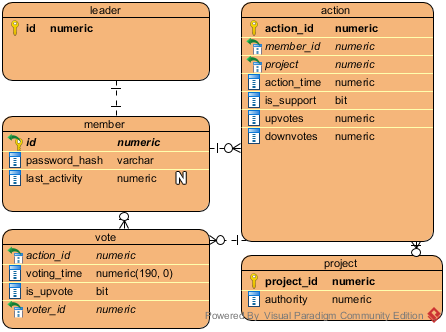
\includegraphics[width=1\textwidth]{er-diagram.png}

\subsection{Więzy i zależności}
Kluczem głównym tablicy \textit{member} jest \textit{id}. Lider wyróżniony jest poprzez istnienie krotki z jego \textit{id} w tablicy \textit{leader}, odwołującej się do \textit{id} członka.\\

\textit{Action} posiada referencję do \textit{member} identyfikującą inicjatora akcji protestu lub wsparcia, oraz do \textit{project} oznaczającą konkretny projekt którego akcja dotyczy.\\

Dane w tabeli \textit{vote} związane są z głosującym \textit{member} oraz \textit{action}.

\subsection{Funkcje pomocnicze}
Zadeklarowałem dwie pomocnicze \textit{SQL}-owe funkcje
\begin{itemize}
	\item \textit{make\_leader(id, password)} dodająca nowego lidera, działająca wyłącznie w trybie --init
	\item \textit{is\_member\_active(id, timestamp)} zwracająca prawdę lub fałsz w zależności od statusu członka
\end{itemize}

\subsection{Opis praw użytkowników init i app}
Użytkownik \textit{init} odpowiedzialny jest za utworzenie tabel, więzów, funkcji oraz pozostałych elementów bazy danych. Musi również przygotować użytkownika \textit{app} i nadać mu odpowiednie prawa, wystarczające do użytkowania świeżo zainicjowanej bazy.\\

Użytkownik \textit{app} posiadać musi minimalny zbiór uprawnień wystarczający do działania, tak aby mógł na przykład odczytać informacje o liderach, lecz nie był w stanie ich zmodyfikować. Operacje \textit{SELECT}, \textit{INSERT} oraz \textit{UPDATE} dostępne są dla tabel \textit{member} (aktualizowanie timestampów) oraz \textit{action} (aktualizowanie liczników).

\subsection{Sposób implementacji funkcji API}
Funkcje wymagające upoważnienia hasłem przed właściwą akcją sprawdzają, czy członek o danym identyfikatorze istnieje, następnie jego hasło i na koniec stan aktywności (czas ostatniej akcji).

\begin{itemize}
	
	\item \textit{open} - to wywołanie musi być podane jako pierwsze po uruchomieniu programu. Wyspecjalizowana klasa odpowiedzialna za pośredniczenie między aplikacją a bazą danych spróbuje nawiązać połączenie, w przypadku niepowodzenia zgłosi błąd, w przeciwnym razie aplikacja przejdzie w stan nasłuchiwania kolejnych poleceń.

	\item \textit{leader} - polega na wywołaniu funkcji \textit{make\_leader(id, password)}, która pod spodem wstawia krotkę do tablicy \textit{member} oraz \textit{leader} oznaczającą członka będącego liderem.

	\item \textit{support protest} - obie funkcje zostaną zaimplementowane jako jedna, a rozpoznawane będą przez flagę \textit{is\_support} w tabeli \textit{action}. W pierwszej kolejności utworzę \textit{project} jeśli nie istniał, upewniając się przy tym, że \textit{authority} zostało podane. Później tworzę wpis w tabeli \textit{action} z detalami zapytania, aktualizuję czas ostatniej aktywności inicjatora.
	
	\item \textit{upvote downvote} - również zaimplementowane jako jedna klasa. Po walidacji danych członka sprawdzam, czy już głosował, jeśli nie, dodaję odpowiednią krotkę do \textit{vote} oraz aktualizuję liczniki w \textit{action}.

	\item \textit{actions} - oprócz sprawdzania poprawności hasła dodatkowo upewniam się, że osoba jest liderem. Zapytanie będzie agregować liczby \textit{upvote} oraz \textit{downvote}, z dodatkowymi obostrzeniami zależnymi od wystąpienia ograniczeń w postaci \textit{type}, \textit{project} czy \textit{authority}.

	\item \textit{projects} - sprowadza się do wypisania danych z tabeli \textit{project}, ewentualnie z ograniczeniem do jednego \textit{authority}.

	\item \textit{votes} - polega na złączeniu tabeli \textit{member} z \textit{action} aby mieć pewność, że uwzględnię również członków którzy nigdy nie głosowali. Zapytanie będzie korzystać z liczników w tabeli \textit{action}.

	\item \textit{trolls} - dzięki redundancji w tabeli \textit{action} nie muszę dynamicznie sumować głosów za i przeciw z tabeli \textit{vote}, co przyspiesza zapytanie. Na tej podstawie trywialnie wyznaczam i odpowiednio sortuję podejrzanych członków, dodając przy tym informację o statusie aktywności.

\end{itemize}

\section{Budowa i uruchamianie aplikacji}

\subsection{Struktura katalogów}
\begin{itemize}
	
	\item \textit{inc} - zawiera pliki nagłówkowe C++.
	
	\item \textit{src} - zawiera pliki źródłowe C++.
	
	\item \textit{resources} - skrypt \textit{init.sql} odpowiedzialny za odpowiednie zainicjowanie bazy w trybie --init, pomocny skrypt \textit{drop.sql} służący do wyczyszczenia bazy do stanu sprzed --init.
	
	\item \textit{documentation} - ten plik pdf.
	
	\item \textit{third\_party} - znajduje się tu open-source'owa biblioteka do parsowania obiektów JSON.
	
\end{itemize}

\subsection{Kompilacja}
Do zbudowania projektu wymagane są system budowania \textit{CMake}, kompilator wspierający standard C++11 oraz oficjalna biblioteka służąca do łączenia z bazą z poziomu kodu C/C++ \textit{libpq}. Program buduję się z włączonymi flagami ostrzeżeń oraz posiada odpowiednie asercje w trybie \textit{Debug}.\\
Polecam utworzyć katalog \textit{build}, wywołać w nim \textit{cmake ..} (CMakeLists.txt znajduje się wtedy w katalogu jeden poziom wyżej). Następnie wykonujemy polecenie \textit{make}, które zbuduje program oraz skopiuje zależności takie jak \textit{init.sql} do katalogu z aplikacją. Program jest gotowy do uruchomienia.

\subsection{Co zostało zaimplementowane}
Działają wszystkie polecenia API. Program zakłada, że pierwszą linią wejścia musi być komenda \textit{open}. W trybie --init dostępna jest wyłącznie funkcja \textit{leader}, wszystkie pozostałe polecenia w trybie ''zwykłym''.
\end{document}